\chapter{Cloud Runtime Environment: Google App Engine}
\label{chap:AppEngine}

An App Engine application is an application that can run on Google Cloud
Platform, which include Linux-based VM instances. The application must be
written in one of the following languages
\begin{itemize}
  \item Java (use Java Runtime Environment)
  \item Python (use fast Python interpreter and standard Python libraries)
  \item PHP
  \item Go (use Go Runtime Environment)
\end{itemize}
\url{https://cloud.google.com/appengine/docs/whatisgoogleappengine}

App Engine gives you 1 GB of data storage and traffic for free, which can be
increased by enabling paid applications.

When your App Engine application is running in the cloud, Google provides a
scalable number of instances of your app's modules. Each instance runs in its
own hosting environment. Initially, it is a sandbox,
Fig.\ref{fig:GoogleCloudPlatform_environment}, containing your code, a webserver
and a language runtime. The language runtime thus was modified to enforce the
sandbox constraints, disabling some of the language APIs (e.g. access
filesystem). Later, Google supports running on Virtual Machine (Managed VM), and
is not restricted to Java and Python runtime environments, e.g. Go runtime
environment or custom runtime
\url{https://cloud.google.com/appengine/docs/managed-vms/custom-runtimes} as
your application is packaged as a Docker container.
When these runtimes are deployed in a Managed VM hosting environment, they support the following service APIs:
\begin{verbatim}
Datastore
Memcache 
Task Queues
Logging
Users
\end{verbatim}

You can also add third-party libraries and frameworks to your app.

You use the existing \verb!app.yaml! (for Python), \verb!appengine-web.xml!
configuration files (for PHP), and App Engine SDK tools to develop and deploy
applications to Managed VMs.

\section{Writing Python apps}

We need \verb!app.yaml! file. For more information, read the Python manual book 
(chapter on Web Framework for Python).

\section{Writing PHP apps}

we need \verb!appengine-web.xml! file. 

\begin{figure}[hbt]
  \centerline{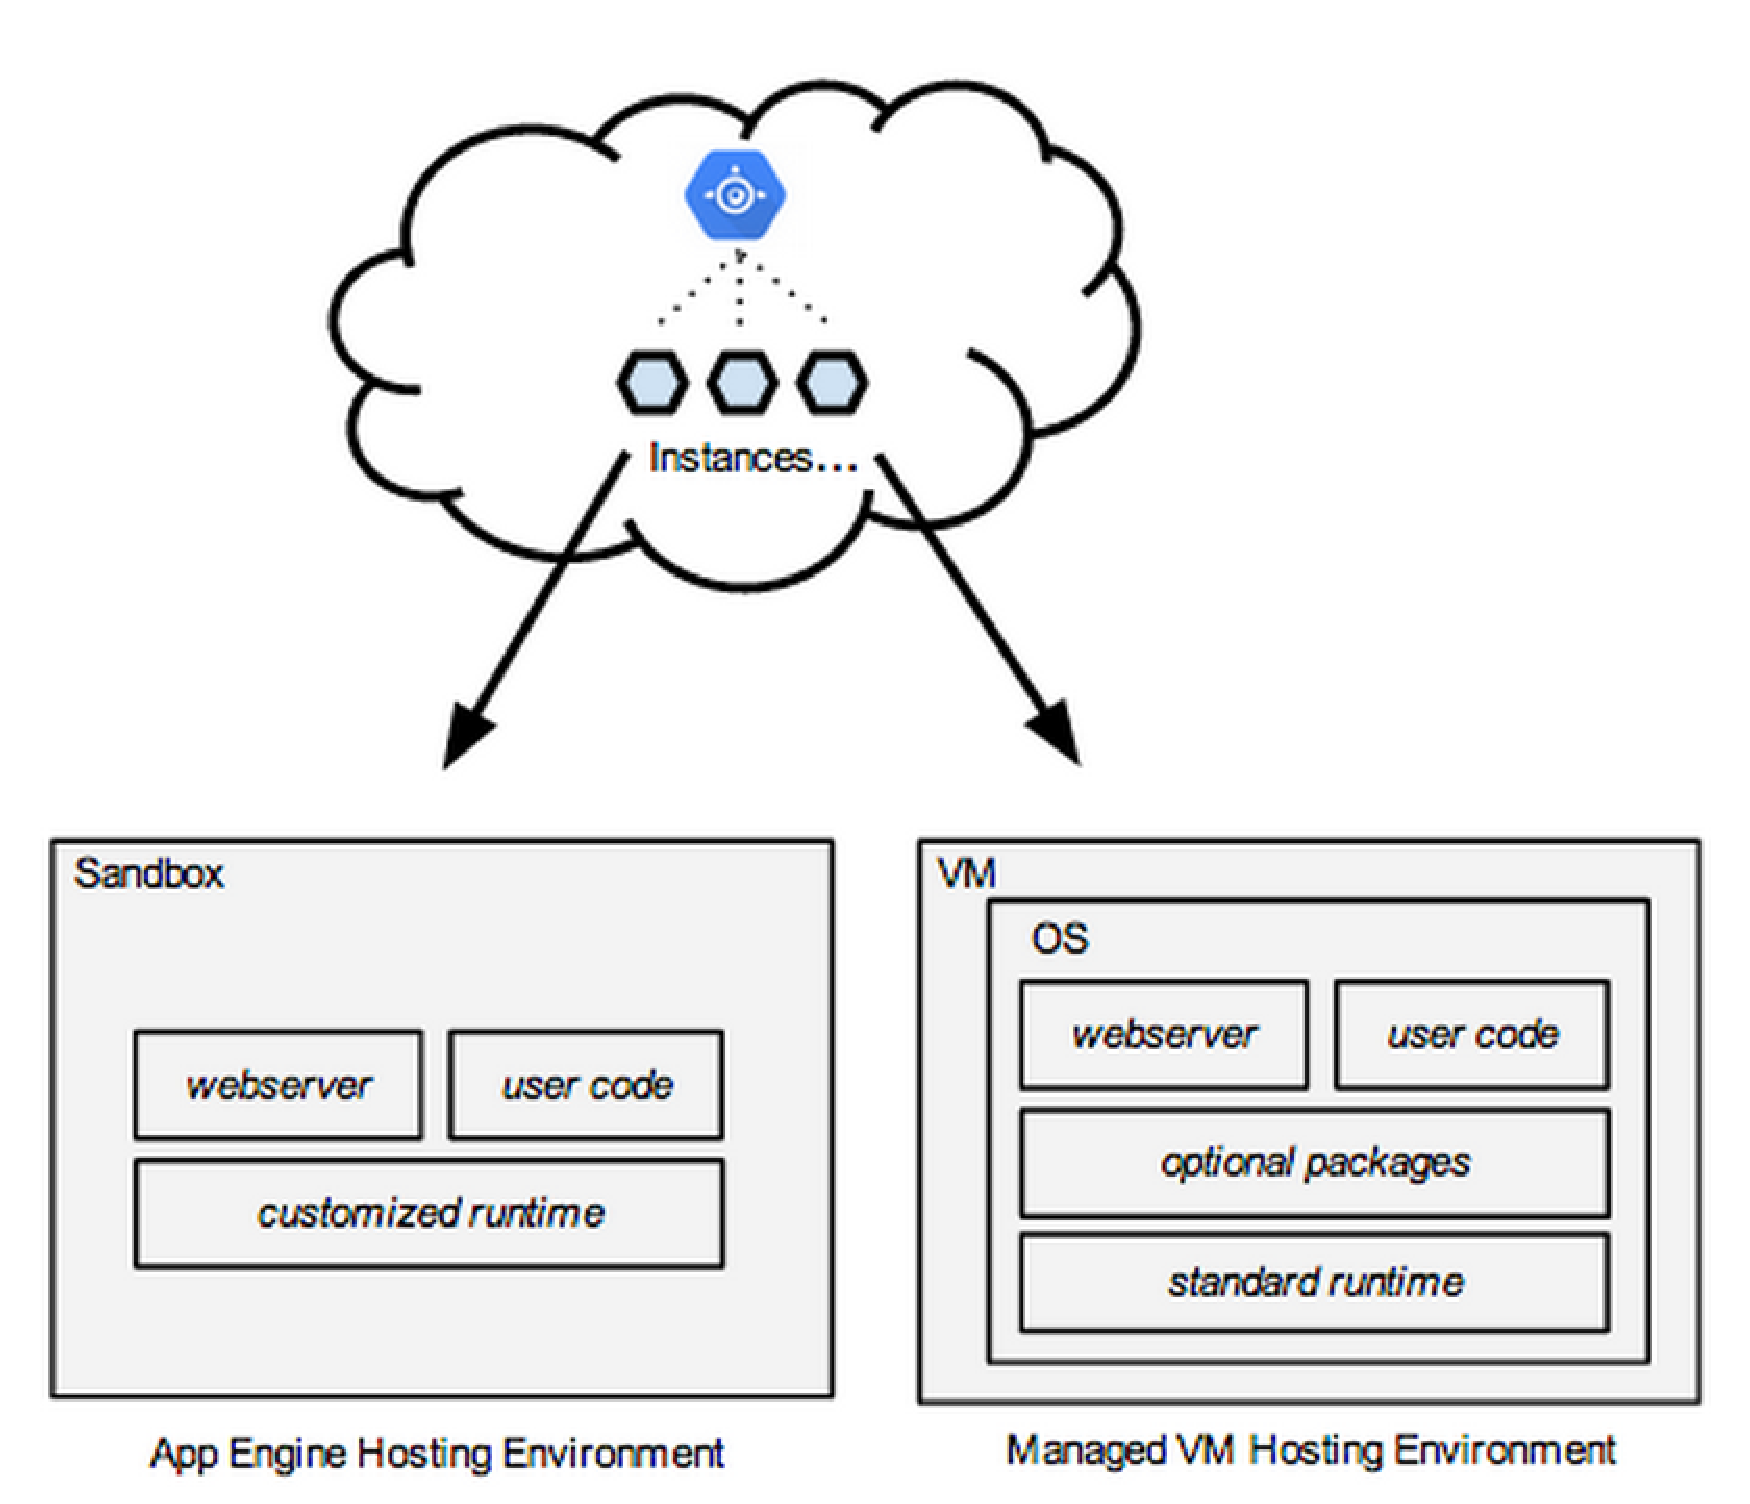
\includegraphics[height=3cm,
    angle=0]{./images/GoogleCloudPlatform_environment.eps}}
  \caption{}
  \label{fig:GoogleCloudPlatform_environment}
\end{figure}


\section{Test your application}

The Launcher is an application for creating, running, uploading, and otherwise
managing Google App Engine applications. 
\url{https://code.google.com/p/google-appengine-wx-launcher/}

\section{Container-as-a-Service}

 The rise of containers and Kubernetes shifted the focus to Containers as a Service (CaaS) from traditional infrastructure services, IaaS. 
 




